\let\negmedspace\undefined
\let\negthickspace\undefined
\documentclass[journal]{IEEEtran}
\usepackage[a5paper, margin=10mm, onecolumn]{geometry}
%\usepackage{lmodern} % Ensure lmodern is loaded for pdflatex
\usepackage{tfrupee} % Include tfrupee package

\setlength{\headheight}{1cm} % Set the height of the header box
\setlength{\headsep}{0mm}     % Set the distance between the header box and the top of the text

\usepackage{gvv-book}
\usepackage{gvv}
\usepackage{algorithmicx} % Ensure algorithmicx is loaded explicitly
\usepackage{cite}
\usepackage{amsmath,amssymb,amsfonts,amsthm}
\usepackage{graphicx}
\usepackage{textcomp}
\usepackage{xcolor}
\usepackage{txfonts}
\usepackage{listings}
\usepackage{enumitem}
\usepackage{mathtools}
\usepackage{gensymb}
\usepackage{comment}
\usepackage[breaklinks=true]{hyperref}
\usepackage{tkz-euclide} 
\usepackage{listings}
% \usepackage{gvv}                                        
\def\inputGnumericTable{}                                 
\usepackage[latin1]{inputenc}                                
\usepackage{color}                                            
\usepackage{array}                                            
\usepackage{longtable}                                       
\usepackage{calc}                                             
\usepackage{multirow}                                         
\usepackage{hhline}                                           
\usepackage{ifthen}                                           
\usepackage{lscape}
\usepackage{algorithm}
\usepackage{algpseudocode}

\renewcommand{\thefigure}{\theenumi}
\renewcommand{\thetable}{\theenumi}
\setlength{\intextsep}{10pt} % Space between text and floats


\numberwithin{equation}{enumi}
\numberwithin{figure}{enumi}
\renewcommand{\thetable}{\theenumi}

% Marks the beginning of the document
\begin{document}
\bibliographystyle{IEEEtran}

\title{10.3.5.1.1}
\author{EE24BTECH11014 - Deepak Ahirwar}

% \maketitle
% \newpage
% \bigskip
{\let\newpage\relax\maketitle}

\textbf{Question:}\\
Check if the given pair of linear equations has unique solution, infinitely many solutions, or no solution. In case there is a unique solution, find it by using cross-multiplication method.
\begin{align}
    x - 3y &= 3\\
    3x - 9y &= 2
\end{align}

\textbf{Solution: }\\

\begin{itemize}
    \item A linear equation is said to be \textbf{consistent} if it has at least one solution.
    \item A linear equation is said to be \textbf{inconsistent} if it has no solution. 
\end{itemize}

Lines represented by the equation
\begin{align}
    a_1x+b_1y &= c_1\\
    a_2x+b_2y &= c_2
\end{align}
are 
\begin{itemize}
\item Intersecting, then
\begin{align}
   \frac{a_1}{a_2} \neq \frac{b_1}{b_2}
\end{align}

\item Coincident, then
\begin{align}
   \frac{a_1}{a_2} = \frac{b_1}{b_2} = \frac{c_1}{c_2}
\end{align}

\item Parallel, then
\begin{align}
   \frac{a_1}{a_2} = \frac{b_1}{b_2} \neq \frac{c_1}{c_2}
\end{align}
\end{itemize}

For our Question, 
\begin{align}
   \frac{a_1}{a_2} &= \frac{1}{3}\\
   \frac{b_1}{b_2} &= \frac{-3}{-9} = \frac{1}{3}\\
   \frac{c_1}{c_2} &= \frac{3}{2}\\
   \frac{a_1}{a_2} &= \frac{b_1}{b_2} \neq \frac{c_1}{c_2}
\end{align}

The system has \textbf{no solution} \\
$\therefore$ It is \textbf{inconsistent}.

\textbf{Cross multiplication method}\\
The cross-multiplication method for solving a system of two linear equations:

is based on the Crammers rule:
\begin{align}
    x = \frac{\mydet{c_1 & b_1\\ c_2 & b_2}}{\mydet{a_1 & b_1 \\ a_2 & b_2}}, \quad y = \frac{\mydet{a_1 & c_1 \\ a_2 & c_2}}{\mydet{a_1 & b_1 \\ a_2 & b_2}}
\end{align}
\begin{align}
& D = \mydet{ 1 & -3 \\ 3 & -9 } = (1)(-9) - (-3)(3) = -9 + 9 = 0 \\
& D_x = \mydet{ 3 & -3 \\ 2 & -9 } = (3)(-9) - (-3)(2) = -27 + 6 = -21 \\
& D_y = \mydet{ 1 & 3 \\ 3 & 2 } = (1)(2) - (3)(3) = 2 - 9 = -7 \\
& x = \frac{D_x}{D} = \frac{-21}{0} \quad \text{(Undefined)}, \quad y = \frac{D_y}{D} = \frac{-7}{0} \quad \text{(Undefined)}\\
\end{align}

Since \( D = 0 \) and \( D_x, D_y \neq 0 \), the system has \textbf{no solution}.

\text{Matrix Method LU Decomposition}
Cnvert the given pair of linear equations into matrix form.\\
We get, 
\begin{align}
    \myvec{1 & -3 \\ 3 & -9 }\myvec{x \\ y} &= \myvec{3 \\ 2}\\
    \Vec{A}x &= \Vec{B} \label{A:}
\end{align}

To solve the above equation, we apply LU - factorization of matrix $\Vec{A}$
We do so, because,
\begin{align}
    \Vec{A} &\mapsto LU\\
    L &\mapsto \brak{\text{Lower triangular matrix}}\\
    U &\mapsto \brak{\text{Upper triangular matrix}}
\end{align}

Let us consider
\begin{align}
    \Vec{U}x = y
\end{align}

Then the equation \eqref{A:} can be written as
\begin{align}
    \Vec{L}y = \Vec{B}
\end{align}

Now the above equation be easily solved using front substitution since $\Vec{L}$ is lower triangular matrix. Thus obtaining a solution for $y$.\\

Now using back substitution in $y = \Vec{U}x$ we can solve for the $x$ since $\Vec{U}$ is a lower triangular matrix.\\

$LU$ factorizing $\Vec{A}$ we get,
\begin{align}
    A &= \myvec{1 & 0 \\ 3 & 1}\myvec{1 & -3 \\ 0 & 0}\\
    L &= \myvec{1 & 0 \\ 3 & 1}\\
    U &= \myvec{1 & -3 \\ 0 & 0}
\end{align}

\textbf{Factorization of LU:}\\
Given a matrix $ \mathbf{A} $ of size $ n \times n $, LU decomposition is performed row by row and column by column. The update equations are as follows: 
\begin{enumerate}
    \item Start by initializing $ \mathbf{L} $ as the identity matrix $ \mathbf{L} = \mathbf{I} $ and $ \mathbf{U} $ as a copy of $ \mathbf{A} $.\\
    \item For each column $ j \geq k $, the entries of $ U $ in the $ k $-th row are updated as:
    \begin{align}
        U_{k,j} = A_{k,j} - \sum_{m=1}^{k-1} L_{k,m} \cdot U_{m,j}\quad \forall \quad j \geq k
    \end{align}
    \item For each row $ i > k $, the entries of $ L $ in the $ k $-th column are updated as:
    \begin{align}
        L_{i,k} = \frac{1}{U_{k,k}} \brak{ A_{i,k} - \sum_{m=1}^{k-1} L_{i,m} \cdot U_{m,k}} \quad \forall \quad i > k
    \end{align}
\end{enumerate}

The solution can be obtained in the following way:

Using forward substitution,
\begin{align}
    \myvec{1 & 0\\ 3 & 1}\vec{y} = \myvec{3 \\ 2}
\end{align}

we get,
\begin{align}
    \vec{y} = \myvec{3 \\ -7}
\end{align}

Now, solving for $\vec{x}$, via backward substitution
\begin{align}
    \myvec{1 & -3 \\ 0 & 0}\vec{x} &= \myvec{3 \\ -7}\\
    \vec{x} &= \text{No solution (Inconsistent system)}
\end{align}

\newpage
\textbf{Algorithms used for LU decomposition:}\\

\textbf{Doolittle Algorithm}
\begin{algorithm}
\caption{Doolittle Algorithm for LU Decomposition}
\label{doolittle}
\begin{algorithmic}[1]
\Require $A$ is an $n \times n$ matrix
\Ensure $L$ is a lower triangular matrix with unit diagonal, $U$ is an upper triangular matrix
\State Initialize $L$ as an $n \times n$ identity matrix
\State Initialize $U$ as an $n \times n$ zero matrix

\For{$k = 1$ to $n$}
    \For{$j = k$ to $n$}
        \State $U_{kj} \gets A_{kj} - \sum_{m=1}^{k-1} L_{km} U_{mj}$
    \EndFor
    \For{$i = k+1$ to $n$}
        \State $L_{ik} \gets \frac{A_{ik} - \sum_{m=1}^{k-1} L_{im} U_{mk}}{U_{kk}}$
    \EndFor
\EndFor

\State \Return $L$, $U$
\end{algorithmic}
\end{algorithm}

\textbf{Crout's Algorithm}
\begin{algorithm}
\caption{Crout's Algorithm for LU Decomposition}
\label{crout}
\begin{algorithmic}[1]
\Require $A$ is an $n \times n$ matrix
\Ensure $L$ is a lower triangular matrix, $U$ is an upper triangular matrix with unit diagonal
\State Initialize $L$ as an $n \times n$ zero matrix
\State Initialize $U$ as an $n \times n$ identity matrix

\For{$j = 1$ to $n$}
    \For{$i = j$ to $n$}
        \State $L_{ij} \gets A_{ij} - \sum_{k=1}^{j-1} L_{ik} U_{kj}$
    \EndFor
    \For{$i = j+1$ to $n$}
        \State $U_{ji} \gets \frac{A_{ji} - \sum_{k=1}^{j-1} L_{jk} U_{ki}}{L_{jj}}$
    \EndFor
\EndFor

\State \Return $L$, $U$
\end{algorithmic}
\end{algorithm}

\begin{figure}[H]
   \centering
   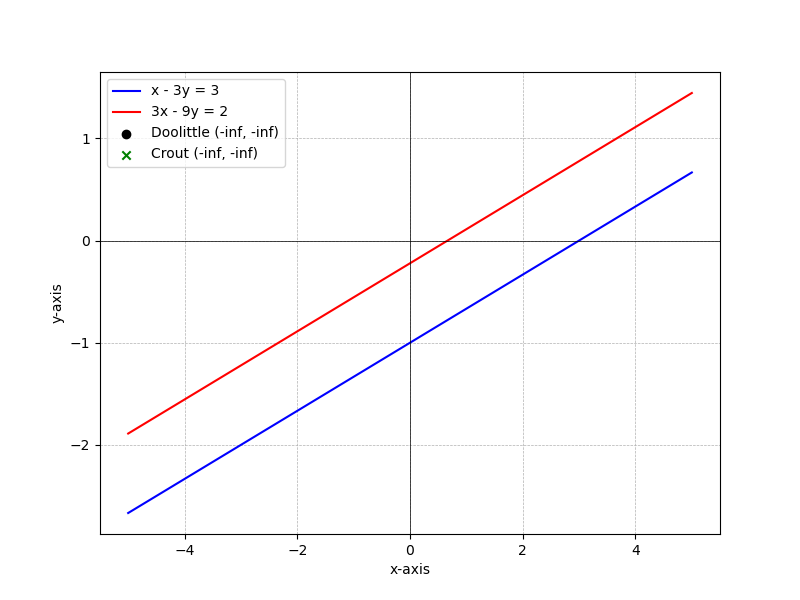
\includegraphics[width=1\columnwidth]{figs/fig.png}
   \caption{Pair of Lines}
\end{figure}


\end{document}
